\newpage\subsection*{1551 Worksheet 8 Answers}
\begin{enumerate}
    
    \item \begin{align*}
     f(x) &= \ln(x-1) \\
     f'(x) &= \frac{1}{x-1} \\
     f'(2) &= 1   
     \end{align*}
	The linearization $L(x)$ near $x = 2$ is
    \begin{align*}
     L(x) &= f(2) + f'(2)(x - 2) \\
     &= ln(1) + (x - 2) \\
     &= x - 2
    \end{align*}
    At $x=3$, $f(3) \approx L(3) = 3 - 1 = 2$. 
    
	\begin{center}
		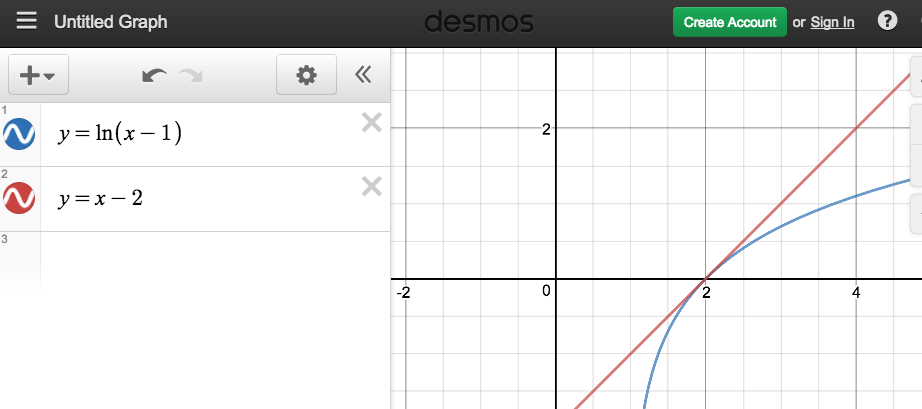
\includegraphics[width=0.8\textwidth]{images/imgWS8ln.png} 
	\end{center}    
    
    
    \item Let $x=x(t)$ be the horizontal distance from wall, $y=y(t)$ is the vertical distance between floor and the top of the ladder. Using the Pythagorean Theorem, when $x$ = 8, $$y = \sqrt{5^2 -4^2} = 3$$
    The Pythagorean Theorem and differentiation gives us
    \begin{align*}
    	5^2 &= x^2 + y^2 \\
        \ddt 18^2 &= \ddt (x^2 + y^2) \\
        0 &= 2x \dxdt + 2y \dydt \\
        0 &= 2\cdot 8 \cdot 3 + 2\cdot 3 \dydt \\
        \dydt &= -8 
    \end{align*}
	The top of the ladder is falling at a rate of 8 ft/s (we could also write this as `the height of the ladder is changing at a rate of -8 ft/s'). \\[12pt] \textit{For full marks, state answer with units}.
    
   \item Use $V = \pi r^2 h$ and differentiate.
   \begin{align*}
   	V &= \pi r^2 h \\
    \ddt V &= \ddt (\pi r^2 h )\\
    V' 
    &= \pi (2rr'h + r^2h')  \\
    &= \pi (2\cdot 5 \cdot r' \cdot 20 + (5)^2h') \\
    &= \pi (200 r'  + 25h') \\
   \end{align*}
   If $D$ is the diameter, and $\frac{dD}{dt} = 1$, then 
   \begin{align*}
   		D&= 2r \\
        \frac{dD}{dt} &= 2 \frac{dr}{dt} \\
        1 &=2 r' \\
        r' &= \frac 1 2
   \end{align*}
   Set $V' = 0$, and solve for $h'(t)$. 
   \begin{align*}
    	0 &= \pi (200 r'  + 25h') \\
    	0 &= \pi (200 \cdot \frac 1 2  + 25h') \\
        h' &= -4
   \end{align*}   
   The height must decrease at a rate of 4 cm/s. 
   
   \item Let $x$ be the side length of the magnet. 
   \begin{align*}
   	\text{volume} = V &= x^3 \\
    dV &= v'(r) \, dr \\
    &= 3r^2 dr \\
    &= 3 \cdot (4)^2 \cdot 0.3 \\
    &= \frac{144}{10} \ \text{cm}^3
   \end{align*}
   The maximum error is 14.4 cm$^3$.
   
   \item 
   \begin{align*}
   		1 &= x^2 + y^2 \\
        0 &= 2x\dxdt + 2y\dydt \\
        \dxdt &= -\frac y x \dydt \\
        &= -\frac{\sqrt 3 /2 }{1/2} (-3) \\
        &=  3\sqrt 3
   \end{align*}
   The $x$-coordinate is changing at a rate of $3\sqrt 3$ units/second.
\end{enumerate}

















